%%%%%%%%%%%%%%%%%%%%%%%%%%%%%%%%%
%
%このファイルは3回のコンパイルの後,
%同梱の./listofcontents.shを用いて
%./listofcontents.sh ファイル名からドットと拡張子を除いたもの
%を1回実行し,最後にもう一度コンパイルをする必要があります.
%
%また,同梱のkanzawa.sty, kanzawa_m.sty, kanzawa2.sty, moreverb.*,
%listofcontents.sh, here.sty, jtygm.sty,
%も必要になります.
%
%
%%%%%%%%%%%%%%%%%%%%%%%%%%%%%%%%%%%
\documentclass[a4j,12pt,dvipdfmx,oneside]{jsbook}
\usepackage{kanzawa2}
\usepackage{here}
\usepackage{times}
\usepackage{amsmath,amsthm,amssymb}
\theoremstyle{definition}
\newtheorem{theorem}{定理}
\newtheorem*{theorem*}{定理}
\newtheorem{Def}[theorem]{定義}
\newtheorem*{Def*}{定義}
\newtheorem{Alg}[theorem]{アルゴリズム}
\newtheorem*{Alg*}{アルゴリズム}
\usepackage{mathptmx}
\usepackage{pifont}
\usepackage{tascmac}
\usepackage{oldgerm}
\usepackage{jtygm}
\usepackage{type1cm}
\setlength{\textwidth}{\fullwidth}
\newcommand{\vd}{\mbox{d}}
\def\rthree{I\kern-2ptI\kern-2ptI}
\newcommand{\namelistlabel}[1]{\mbox{#1}\hfil}
\newenvironment{namelist}[1]{
	\begin{list}{}
		{\let\makelabel\namelistlabel
		\settowidth{\labelwidth}{#1}
		\setlength{\leftmargin}{1.1\labelwidth}}
}{
\end{list}}

\usepackage[T1]{fontenc}
\usepackage{textcomp}
\usepackage[utf8]{inputenc}
\usepackage{lmodern}
\usepackage[all, warning]{onlyamsmath}
\kanjiencoding{JY1}
\kanjifamily{mc}
\kanjiseries{m}
\kanjishape{n}
\selectfont
\usepackage{enumitem}
\newcommand{\argmax}{\operatornamewithlimits{\mathrm{arg\,max}}}
\newcommand{\argmin}{\operatornamewithlimits{\mathrm{arg\,min}}}
\newcommand{\QED}{\hfill$\blacksquare$\par}
\usepackage{longtable}
\usepackage[dvipdfmx]{graphicx}
\usepackage{mediabb}
\makeatletter
\def\minimize{\mathop{\operator@font minimize}} 
\makeatother
\usepackage{eclbkbox}	% required for `\breakbox' (yatex added)
\begin{document}
\pagestyle{headings}
\def\thepage{\roman{page}}
\input epsf
\tableofcontents
\listoffigures
\listoftables
%%%%%
\newpage
\pagestyle{myheadings}
%
%
%
\chapter{序論}
\def\thepage{\arabic{page}}
\setcounter{page}{1}
\label{chap:first}
%
%
%
\section{背景}\label{sec:background}
%
%
%
\subsection{ファジィクラスタリング}\label{subsec:latex}
%
%
%

%
%
%
\subsection{クラスタサイズ調整変数}\label{subsec:academic_statement}
%
%
%

%
%
%
\section{目的}\label{sec:purpose}
%
%
%

%
%
%
\section{構成}\label{sec:contents}
%
%
%
本文書の構成を次に示します.
第\ref{chap:checkManuscript}章では,指導教員に原稿を校正させることについて
説明しています.
第\ref{chap:abst}章では,卒業論文概要書作成について
説明しています.
第\ref{chap:thesis}章では,卒業論文作成について
説明しています.
第\ref{chap:presen}章では,発表資料作成について
説明しています.
第\ref{chap:statement}章では,卒業論文概要書,卒業論文,および発表資料に盛
り込まれる文章について
説明しています.
最後に第\ref{chap:conclusion}章では,本文書の結論を述べています.
また,付録では,
原稿チェックリスト,過去の卒業研究中間発表会と卒業研究発表における配布資
料を掲載してます.
%
%
%
\chapter{実験内容}\label{chap:checkManuscript}
%
%
%
\section{はじめに}\label{sec:checkManuscript_intro}
本章では,卒業論文概要書や卒業論文などの作成した文書を指導教員に校正させ
る上での注意点が書かれています.
まず第~\ref{sec:checkManuscript_abst}節でその概要を示し,
次に第~\ref{sec:checkManuscript_misc}節でその他の注意点を示しています.
%
%
%
\section{概要}\label{sec:checkManuscript_abst}
%
%
%
\section{そのほかの注意}\label{sec:checkManuscript_misc}
%
%
%
\section{おわりに}\label{sec:checkManuscript_summary}
本章では,卒業論文概要書や卒業論文などの作成した文書を指導教員に校正させ
る上での注意点を述べました.
まず第~\ref{sec:checkManuscript_abst}節でその概要を示し,
次に第~\ref{sec:checkManuscript_misc}節でその他の注意点を示しました.
%
%
%
\chapter{卒業論文概要書作成}\label{chap:abst}
%
%
%
\section{はじめに}\label{sec:abst_intro}
本章では,卒業論文概要書の作成について述べます.
まず第\ref{sec:abst_feature}節で卒業論文概要書の性格を示します.
次に第\ref{sec:abst_flow}節で作業の流れを示します.
最後に第\ref{sec:abst_file}節でサンプルファイルの扱いを示します.
%
%
%
\section{卒業論文概要書の性格}\label{sec:abst_feature}
卒業論文概要書は,本体である卒業論文の要約であり,
それを一読して当該卒業研究の目的と成果が
理解され得なければなりません.
例えば3年生は,
卒業論文概要集を読んで各研究室の卒業研究内容を把握しようとしているようですが,
3年生が皆さんの書いた概要集を読んで,
「神澤研にいきたい!」
って思うかどうかは別にして,
少なくとも,
「神澤研ではこんなことをやってるんだぁ.じゃここにいく事はないね」
と判断がつかなければなりません.
ちなみに,難解な数式を並べたことによって,
「訳分からないからここにいく事はないね」
っていうのはなしです(結論は同じだけど).
勿論,本来,卒業論文概要書は卒業論文の概要という,
卒業論文に付随した公式文書であって,
決して3年生の研究室配属に際しての参考資料のためにあるのではありませんが,
「3年生が分かるように」というのは,
良い目安だと思います.

その一方で,卒業論文概要書はそれ自体で閉じていなくてはならず,
文中の記号や専門用語は当該文書内で定義しなくてはなりません.
決して,「分からなければ本体の卒業論文読んでね」ではダメです.
でも,自分の研究内容を正確に書いていくと,
あっという間に紙面は埋まってしまいます.
もし埋まらなかったら,内容をはしょり過ぎてるってこと.
一度,文章に登場した記号や用語はちゃんと説明しなきゃいけない一方で,
紙面が限られているという制約条件.
実は,卒業論文本体の作成よりも卒業論文概要書作成の方が難しいのです.

そのため,細かい議論は避け,成果を代表する図表を使うことをお勧めします.
当研究室の研究内容は数学的議論が多いため,
定義と定理と数式を書き並べて紙面を埋める卒業論文概要書になりがちですが,
数理の武装で逃げずに,文章で説明するよう努力しましょう.
%
%
%
\section{作業の流れ}\label{sec:abst_flow}
%
%
%
以下に,理想的な作業の流れを示しています.
特に第1, 2, 3小節については,これが理想であることを踏まえて
現実的に対応して下さい.
\subsection{紙面上での定式化}
まず,基となる研究内容を定式化します.
ここで正しくかつ厳密に定式化しておかないと,
後の卒業論文作成・発表資料作成・発表練習時に苦労します.
期限が迫っているからといって,定式化せずに次の作業に移らないでください.
ここで定式化しておけば,後が楽になります.
次の作業が終わる前に指導教員に確認を得て下さい.
%
%
%
\subsection{定式の文章化}
%
%
%
数式などを用いて定式化しておいたものを日本文にしていきます.
一般に,数式を日本文にすることは至難の技ですが,
可能な限り,数式の本質を文章化します.
どうしても日本文にできないものはしかたないので,数式をそのまま使いますが,
どうしても日本文にできない数式のほとんどは研究内容の本質を表すものではなくて
瑣末なものです.つまり「概要」には不要ということになります.
ここで分量や見栄えには拘らないべきです.
内容が定まらないままにこれらに拘り始めると作文の本質を見誤ることになります.
文章作成に関しては第~\ref{chap:statement}章を,
数式に関しては第~\ref{chap:math}章を読み,慎重に校正して下さい.
数値実験に関しては第~\ref{chap:experiment}章を読み,必要事項を明記して下さい.
予め,必要事項を明記できるように実験データをとっておいて下さい.
参考文献は,第~\ref{chap:cite}章を読み,
当文書の参考文献の記述を参考にして下さい.
%
%
%
%
\subsection{紙面上での「構成」の構成}
構成を練ります.
「まえがき」「あとがき」「数値例」「参考文献」は必須です.
「まえがき」と「あとがき」の間に本論が入ることになります.
本論を\ruby{一}{ひと}章にするか,さらに章分けするかは本章の内容に依存しますが,
分量の制約から\ruby{一}{ひと}章にする可能性が高いでしょう.
次の作業が終わる前に指導教員に確認を得て下さい.
%
%
%
\subsection{\LaTeX{}化}
構成を練り終わったら,その構成に基づいて文章を作成します.
まず,
分量やレイアウトに拘らず,
\LaTeX{}を用いて活字化することによる見栄えを気にします.
文章作成に関しては第~\ref{chap:statement}章を,
数式に関しては第~\ref{chap:math}章を読み,慎重に校正して下さい.
次の作業に入る前に指導教員に判断を仰いで下さい.
%
%
\subsection{仕上がりレイアウトや分量の調整}
文字は勿論のこと,図表や数式の全てが印字範囲内に収まっていることを確認し
て下さい.
数式が行幅を超えている場合には,複数行に分けることを検討しましょう.
図が行幅を超えている場合には,図を縮小することになると思いますが,
図内に埋め込まれた文字が,本文中の下付き文字の大きさと同じかそれより大き
いことを確認して下さい.
そうでない場合には作図作業から始めた方がいいかもしれません.
表が行幅を超えている場合に,安直に文字サイズを変更しようとせず,
まずは表レイアウトの妥当性について再度,検討しましょう.
どうしても文字サイズを縮小せざるを得ない場合には
予め指導教員に確認して下さい.
また,本文中の標準文字サイズ(題目の文字サイズや本文中の上付きや下付きで
ない文字のサイズ)を変更しないで下さい.

自分の文書が指定分量に満たない場合には内容が貧弱すぎるので,
もう一度前の作業に戻ります.
指定分量を越える場合には当然,内容を減らさなければなりませんが,
何を減らすかについては指導教員の指示に従って下さい.
ほとんどの場合,単純にある部分を削除することにはなりません.
ここでもう一度,文章や数式を練り直します.
%
%
%
\subsection{提出前の確認}
内容・レイアウト・分量について指導教員から提出許可を得たら,
提出作業に入りますが,ここでもう一度,提出ファイルについて,
全てのフォントが埋め込まれていること,
用紙サイズがA4ポートレートであること,および,
ファイル名が指定にしたがっていることを確認して下さい.
また,締め切り直前に思わぬ事故が発生することもあるため,
提出は期限前に余裕を持つことを心がけて下さい.
%
%
%
\section{ファイル操作}\label{sec:abst_file}
%
%
%
あらかじめサンプルファイル\texttt{sample.tex}とスタイルファイル
\texttt{style.cls}をダウンロードし,
サンプル\LaTeX{}ファイルから,次の通りにPDFファイルを作成します.
\begin{enumerate}
\item 通常通りのコンパイル
\item { }
\begin{center}
\texttt{dvipdfmx -f \~/ipaex.map -d 5 sample.dvi}
\end{center}
によってpdfファイルを得ます.
\item { }
\begin{center}
\texttt{evince sample.pdf}
\end{center}
で印刷仕上がりを確認できます.Alt+Enterで,
用紙サイズがA4であることと,全フォントが埋め込まれていることを確認して下
      さい.
\end{enumerate}
%
%
%
\section{おわりに}\label{sec:abst_summary}
本章では,卒業論文概要書の作成について述べました.
まず第\ref{sec:abst_feature}節で卒業論文概要書の性格を示しました.
次に第\ref{sec:abst_flow}節で作業の流れを示しました.
最後に第\ref{sec:abst_file}節でサンプルファイルの扱いを示しました.
%
%
%
\chapter{卒業論文}\label{chap:thesis}
%
%
%
\section{はじめに}\label{sec:thesis_intro}
本章では,卒業論文の作成について述べます.
まず第\ref{sec:thesis_contents}節で卒業論文の構成を示します.
次に第\ref{sec:thesis_examples}節で卒業論文をより充実したものにするため
の工夫について示します.
最後に第\ref{sec:thesis_file}節でサンプルファイルの扱いを示します.
%
%
%
\section{構成}\label{sec:thesis_contents}
第一章は序論.背景・目的・構成が書かれます.
例えば,第一節を背景・第二節を目的・第三節を構成とします.
さらに細かく分けたいときには「小節」を用います.
背景については図表をカウントしないで2ページ目に及ぶように文章量を稼いで下さい.

ここで,章立てとそのラべリングについて述べておきます.
\LaTeX は参照機能を有しており,それを積極的に用いるべきです.
参照機能は特に,数式や参考文献の参照においてその威力を発揮しますが,
章立てにも参照機能を用いるべきです.\LaTeX における章立は,
\begin{verbatimtab}
\{chapter}{章の名前}
\{section}{節の名前}
\{subsection}{小節の名前}
\end{verbatimtab}
のように行われますが,以下のようにそれぞれにラベルをつけておきます.
\begin{screen}
\begin{verbatimtab}
\{chapter}{章の名前}\label{chap:korekore}
\{section}{節の名前}\label{sec:kakukaku}
\{subsection}{小節の名前}\label{subsec:shikajika}
\end{verbatimtab}
\end{screen}
実際,本章には\texttt{sec:thesis\_contents}なるラベルがつけられています.
これによって,章(節,小節)番号を参照するときに,
\begin{screen}
\begin{verbatimtab}
第~\ref{sec:thesis_contents}節においては$\cdots$
\end{verbatimtab}
\end{screen}
とタイプしておくと,
\begin{screen}
第~\ref{sec:thesis_contents}節においては$\cdots$
\end{screen}
と印刷されることになります.
このラべリングと参照は一見面倒に感じますが,
後になって,新しい章をどこかに挿入することによって章番号がずれても
本文中の参照個所を全てチェックしなくても良いという利点があります.
参照個所のミスは見つけにくい一方で,読者にとっては真に腹立たしいミスであり,
絶対避けるべきであるため,この参照機能使用を義務とします.
尚,上の例ではラベル名を,
\texttt{chap:korekore}のように「章コマンドの略称:名前」のようにしています.
一般には第一文字が英字で以後は英数字,ハイフン`\texttt{-}', アンダーバー`\texttt{\_}'であれば良い
(厳密には他の文字も許されるかも知れないが運用上はないと言って良い)のですが,
ラベル名が重複してはいけないことと,
参照時に何を参照しているかを容易に思い出せるようにするために,
上例のような命名を勧めます.
第~\ref{chap:reference}章も読んで下さい.

第二章以降は準備.題目は各章の内容に従います.
ここで,記号・方法の定義を行います.アルゴリズムは,
\begin{verbatimtab}
\begin{Alg}[題目]
アルゴリズムの内容
\end{Def}
\end{verbatimtab}
のように書きます.
その他,定義・定理・例・補題も同様の形式とします.
それぞれの,書式は同梱の\texttt{kanzawa.sty}を参照して下さい.
これらを「環境」といいます.「環境」の前に,その「環境」の説明を述べます.
例えば,
\begin{screen}
標準的ファジィ$c$-平均法~(Standard Fuzzy $c$-Means: sFCM)は,
次のアルゴリズムにしたがう:
\begin{Alg}[sFCM]~\cite{kanzawa}
\begin{enumerate}[label=\textsc{Step}~\arabic*., labelindent=\parindent, leftmargin=*]
\item
ファジィ化パラメータ$m>1$を設定し,
初期クラスタ中心$\{v_i\}_{i=1}^C$を設定する.
\label{sFCM:enum:initialize}
\item
オブジェクト-クラスタ間非類似度$\{d_{i,k}\}_{(i,k)=(1,1)}^{(C,N)}$を
次のように設定する:
\begin{align}
d_{i,k}=\|x_k-v_k\|_2^2.
\end{align}
\label{sFCM:enum:dissimilarities}
\item
帰属度$\{u_{i,k}\}_{(i,k)=(1,1)}^{(C,N)}$を次のように設定する:
\begin{align}
u_{i,k}=
\frac{1}{\sum_{j=1}^C\left(\frac{d_{i,k}}{d_{j,k}}\right)^{1/(m-1)}}
\end{align}
\label{sFCM:enum:membership}
\item
クラスタ中心$\{v_i\}_{i=1}^C$を次のように設定する:
\begin{align}
 v_i=\frac{\sum_{k=1}^N{}(u_{i,k})^m{}x_k}{\sum_{k=1}^N{}(u_{i,k})^m}.
\end{align}
\label{sFCM:enum:centers}
\item
$(u,v)$が収束すれば終了,そうなければ\ref{sFCM:enum:dissimilarities}へ.\QED
\end{enumerate}
\end{Alg}
本アルゴリズムでは初期設定としてクラスタ中心を与えているが,
初期帰属度を設定して,クラスタ中心,オブジェクト-クラスタ間非類似度,帰
 属度の順に設定することもできる.
\end{screen}
の通り.ここで注意すべきは,アルゴリズム全体で大きな文字として解釈し,そ
の終わりが句点「.」の代わりに「$\blacksquare$」が使われていること.そして,
次に続く文が前のアルゴリズムを補足するものであるために改段落せずに続いて
いること.もし,アルゴリズムの後に,異なる内容を記述する場合には,
\LaTeX{}ソース内で空行を設けて,改段落すること.

準備に相当する章を単一とするか複数の章に分けるかについてはその内容に依存します.

第二章以降,結論に相当する章まではすべて,
第一節を「はじめに」,最終節を「おわりに」とし,各節でその章の要約を述べます.

次は主題.題目は内容に従います.
主題に相当する章を単一とするか複数の章に分けるかはその内容に依存します.
ここでは仮に,eFCMが提案手法であると仮定して,その導出からアルゴリズム記載までの例を示します.
\begin{breakbox}
HCMは,帰属度の制約を$\{0,1\}$から$[0,1]$に緩和してもなお,
最適解は$\{0,1\}$のいずれかになる.
これを特異な状態であるとして正則化することを考える.
正則化項を帰属度に関する負のShannonエントロピーとすると次の最適化問題が得られる:
\begin{align}
&\minimize_{u,v}\sum_{i=1}^C\sum_{k=1}^Nu_{i,k}\|x_k-v_i\|_2^2
+\lambda^{-1}\sum_{i=1}^C\sum_{k=1}^Nu_{i,k}\log(u_{i,k})
\label{eq:eFCM-objective}\\
&\text{subject to }\sum_{i=1}^Cu_{i,k}=1.
\label{eq:eFCM-constraint}
\end{align}
ここで,$\lambda>0$は正則化の度合いを調整するためのファジィ化パラメータである.
この最適化問題を解くことによって得られる手法をエントロピー正則化ファジィ$c$-平均法~(entropy-regularized fuzzy $c$-means: eFCM)と呼ぶ.
最適化問題~(\ref{eq:eFCM-objective}), (\ref{eq:eFCM-constraint})に対応するLagrange関数$L_{\mathsf{eFCM}}(u,v,\gamma)$は次のように表される:
\begin{align}
 L_{\mathsf{eFCM}}(u,v,\gamma)=& \sum_{i=1}^C \sum_{k=1}^N 
 u_{i,k} \|x_k-v_i\|_2^2
+\lambda^{-1}\sum_{i=1}^C\sum_{k=1}^Nu_{i,k}\log(u_{i,k})\notag\\
&+\sum_{k=1}^N\gamma_k\left(1-\sum_{i=1}^Cu_{i,k}\right).
\end{align}
ここで$\gamma=(\gamma_1,\dots,\gamma_N)$はLagrange乗数である.
最適性の必要条件は次のように表される:
\begin{align}
 \frac{\partial{}L_{\mathsf{eFCM}}(u,v,\gamma)}{\partial{}u_{i,k}}=&0,\label{eq:eFCM-membership-condition}\\
 \frac{\partial{}L_{\mathsf{eFCM}}(u,v,\gamma)}{\partial{}v_i}=&0,\label{eq:eFCM-centers-condition}\\
 \frac{\partial{}L_{\mathsf{eFCM}}(u,v,\gamma)}{\partial{}\gamma_k}=&0.\label{eq:eFCM-gamma-condition}
\end{align}
最適な帰属度$\{u_{i,k}\}_{(i,k)=(1,1)}^{(C,N)}$は
条件式~(\ref{eq:eFCM-membership-condition})によって
Lagrange乗数$\gamma_k$を用いて次のように表される:
\begin{align}
&d_{i,k}+\lambda^{-1}\left(\log(u_{i,k})+1\right)-\gamma_k=0\notag\\
\Leftrightarrow&u_{i,k}=\exp(\gamma_k-1-\lambda d_{i,k}).
\label{eq:eFCM-membership0}
\end{align}
ここで,$d_{i,k}=\|x_k-v_i\|_2^2$である.
条件式~(\ref{eq:eFCM-gamma-condition})を考慮して
式~(\ref{eq:eFCM-membership0})をクラスタインデックス$j\in\{1,\cdots,C\}$について総和をとると帰属度の更新式を次のように得る:
\begin{align}
u_{i,k}=\frac{
 \exp(-\lambda d_{i,k})
}{
 \sum_{j=1}^C\exp(-\lambda d_{j,k})
}.
\label{eq:eFCM-membership}
\end{align}

最適なクラスタ中心$\{v_i\}_{i=1}^C$は
条件式~(\ref{eq:eFCM-centers-condition})によって
次のように表される:
\begin{align}
&2\sum_{k=1}^Nu_{i,k}(x_k-v_i)=0\notag\\
\Leftrightarrow&v_i=\frac{\sum_{k=1}^Nu_{i,k}x_k}{\sum_{k=1}^Nu_{i,k}}.
\label{eq:eFCM-centers}
\end{align}
以上より,eFCMは次のアルゴリズムにまとめられる:
\begin{Alg}[eFCM]~\par
 \label{alg:eFCM}
\begin{enumerate}
\setlength{\itemindent}{3em}
\renewcommand{\theenumi}{\arabic{enumi}}
\renewcommand{\labelenumi}{\textsc{Step~\theenumi.}}
\item
クラスタ数$C$,
ファジィ化パラメータ$\lambda>0$,
初期クラスタ中心$v$を設定する.
\item
個体-クラスタ間非類似度$\{d_{i,k}\}_{(i,k)=(1,1)}^{(C,N)}$を次のように計算する:
\begin{align}
d_{i,k}=\|x_k-v_i\|_2^2.\label{eq:eFCM-dissimilarities}
\end{align}
\item
帰属度$u$を次のように計算する:
\begin{align}
u_{i,k}=\frac{
 \exp(-\lambda d_{i,k})
}{
 \sum_{j=1}^C\exp(-\lambda d_{j,k})
}.
\label{eq:eFCM-membership1}
\end{align}
\item
組$(u, v)$の停止条件を確認する.
もし条件を満たせば終了,そうでなければStep.~2へ.\QED
\end{enumerate}
\end{Alg}
\end{breakbox}



主題の章の後に,数値例の章.詳しくは第~\ref{chap:experiment}章を参照して下さい.

次は結論.各章別に何を記したのかと残された課題を書きます.

次は参考文献.詳細は第~\ref{chap:cite}章を参照して下さい.

次に感想.
研究を遂行してきた際,何につまづき,何は難しかったかを書きます.
章立てしませんが目次には掲載します.
ここは余程のことがない限り校正しませんが,
後輩達のために,いっぱい書いて下さい.
指導教員への文句でも構いません.

次に謝辞.
謝辞には,研究遂行に当たって感謝すべき人間に感謝の言葉を記します.
くじけそうになったときに励ましてくれた友人や家族も.
章立てしませんが目次には掲載します.
ここも余程のことがない限り校正しません.

最後に付録.
数値例に用いたプログラムソースを全て掲載します.
ただし,無意味なコメントなどを削除し,
プログラムの各所に説明のコメントをつけて下さい.
後輩達がそれを見て,何をしている部分なのかが直ぐ分かるようにして下さい.
章立てしませんが目次には掲載します.
%
%
%
\section{例・イメージ描写・表・図を豊富に}\label{sec:thesis_examples}
%
%
%
卒業論文を論文として見た場合,
背景から結論までの内容,
記号や用語の定義,実験結果や定理などの研究成果が明記されていれば,
一応の体裁が整ったことになります.
その一方で,卒業論文は後輩が卒業研究を遂行する上での
教科書としての側面も持ちます
(皆さんも先輩方の卒業論文を参考にしていますよね).
学術的な厳密さだけでは教科書として成り立ちません.
ある定義を記述したら,その後に,その定義に関する理解を深めるための
例やイメージ,場合によっては表や図を駆使して,
読者の理解を助ける努力をして下さい.
一つの考え方として,発表資料作成に用いた概念図を全て卒業論文に盛り込むと
よいでしょう.勿論その際には,図を本文中で引用し,
引用文として発表の際の口頭説明を論文用に書き下すとよいでしょう.
また,皆さんが今までに出会った,
良いと感じた教科書と悪いと感じた教科書を比べ,
自分の卒業論文が良い教科書になるように努力して下さい.
%
%
%
\section{必要ファイルの入手}\label{sec:thesis_file}
%
%
%
卒業論文作成に必要なファイルは
\begin{center}
\texttt{http://www.kanz.ce.shibaura-it.ac.jp/lab/}
\end{center}
から入手可能です.
\texttt{thesis-*.*.tgz}をホームディレクトリのどこかにダウンロードして下さい.
ここで\texttt{*.*}はバージョン番号を表します.
最新バージョンをダウンロードして下さい.
\begin{screen}
\texttt{tar xvfz thesis-*.*.tgz}
\end{screen}
でディレクトリ\texttt{thesis-*.*}以下にファイルが展開されます.

コンパイル作業に入る前に,同梱の\texttt{listofcontents.h}に対して
\begin{screen}
\texttt{chmod 755 listofcontents.sh}
\end{screen}
としておきます.
%
%
%
\subsection{\texttt{thesis\_sample.tex}について}\label{sec:thesis_sample}
このファイルは卒業論文作成にあたって清書に用いるファイルです.
ただし,表紙は別に\texttt{titlepage.tex}を用います.

以下の通りにコンパイル作業を行います.
\begin{enumerate}
\item 通常通りのコンパイルを3回行います.
このとき,
logファイルにエラーメッセージや警告メッセージがないことを確認して下さい.
\item { }
\begin{center}
\texttt{./listofcontents.sh thesis\_sample}
\end{center}
とします.
\item もう一度コンパイルを行います.
このとき,
logファイルにエラーメッセージや警告メッセージがないことを確認して下さい.
\end{enumerate}
\begin{center}
\texttt{dvipdfmx -f ~/ipaex.map -d 5 thesis\_sample.dvi}
\end{center}
として,ファイル\texttt{thesis\_sample.pdf}を得ます.

本文書の指示には勿論したがって貰いますが,
本文書のソースファイル\texttt{thesis\_sample.tex}の中身と印刷物を比較しながら
卒業論文を作成して下さい.
%
%
%
\subsection{\texttt{titlepage.tex}について}\label{sec:titlepage}
%
%
%
このファイルは卒業論文表紙作成にあたって清書に用いるファイルです.

通常のコンパイルと
dvipdfmxコマンドにより印刷を行なうことができます.

本文書の指示には勿論したがって貰いますが,
本文書のソースファイル\texttt{thesis\_sample.tex}の中身と印刷物を比較しながら
卒業論文を作成して下さい.
%
%
%
\section{おわりに}\label{sec:thesis_summary}
本章では,卒業論文の作成について述べました.
まず第\ref{sec:thesis_contents}節で卒業論文の構成を示しました.
次に第\ref{sec:thesis_examples}節で卒業論文をより充実したものにするため
の工夫について示しました.
最後に第\ref{sec:thesis_file}節でサンプルファイルの扱いを示しました.
%
%
%
\chapter{発表資料作成}\label{chap:presen}
%
%
%
\section{はじめに}\label{sec:presen_presen}
本章では,発表資料の作成について述べまます.
まず第\ref{sec:presen_intro}節で発表資料作成における理想的な心構えを示します.
次に第\ref{sec:presen_make}節で発表資料の理想的な作成手順を示します.
%
%
%
\section{概論}\label{sec:presen_intro}
%
%
%
本節では,発表資料作成における理想的な考え方を説明しています.
これが理想であることを踏まえて現実的に対応して下さい.

とりあえず,作り始めるのではなく,
まずはどのような流れで発表するのかを良く考えて下さい.

時間は8分.この時間で何も分からない人達に,
自分の研究の目的・内容・結果を理解して貰わなければなりません.
半年近い時間をかけて理解してきたことを8分で理解させるのだから,
大胆かつ慎重な取捨選択が必要となります.

まずは,「自分の研究を一言で言えば何なのか?」の答えを用意します.
もし,専門用語を使って説明したのであれば,
その専門用語は何を意味するのかを説明しなければなりません.
仮にこの質問の問いに聴衆が理解したとして,
聴衆には次の疑問が生れます.
「それは何のためにやっているのか?」
「結局,何をしたのか?」
「研究の成果はどうだったのか?」,
「他人による同一研究との比較は?」
「オリジナリティはどこにあるのか?」,
「残された研究課題は何か?」
それぞれに一言の答えを用意し,
その一言に聴衆が理解できないと思われる場合には,
さらに一言を加えていきます.

ドラマチックな発表を!そのために技を使います.
	
細かいことは話しても分かって貰えません.

発表は論文のような公式資料ではないため,特別に決まった形式はありません.
これは,ルールや慣習に縛られない自由がある反面,
これで及第するといった基準がないことを意味します.
あまりに自由すぎると却って困るのか,
平々凡々とした発表に陥りやすくなります.

発表資料が何も無い状態で発表することを想像してみて下さい.
式,図や表がなく,言葉だけで説明することが難しい
ことが分かると思います.
そのような情報(式・図・表)をプレゼン資料に入れていきます.
覚えられない論理展開やセリフをプレゼン資料に入れていってはいけません.
%
%
%
\section{作成手順}\label{sec:presen_make}
%
%
%
本節では,発表資料作成における理想的な作成手順を説明しています.
これが理想であることを踏まえて現実的に対応して下さい.
\begin{enumerate}
\item 発表シナリオをA4サイズ紙面1枚程度にまとめます.
シナリオはセリフを書いたものではないことに注意して下さい.
\item シナリオ\underline{だけ}を用いて,声に出して,
発表に相当する練習を行い,随時,シナリオを修正していきます.
ここで発表時間は気にしないで下さい.
気にすべきことは,論理的思考に基づいて,
不足内容を,
分かりやすく,
正しい日本語を用いた説明ができるか否かです.
発表しづらい場合は,シナリオが練り切れていない可能性が非常に高いです.
シナリオを練り直して下さい.
また,論文内の誤りに気づいた場合は,論文も修正して下さい.
\item 指導教員から許可を得たものに限り,
シナリオを基に,発表資料に相当するものを,
手書きでA4, Landscapeで作成します.
複数行に渡る文章がないよう注意して下さい.
矢印を多用しないで下さい.
矢印を多用するとさっさと発表資料を作れますが,
それを見る聴講者はさっぱり分からないと思います.
それは,著者の使った矢印には各所で微妙に異なる意味が込められているからです.
その意味を明らかにすると,自然と矢印は消えていきます.
また,矢印を使用する場合は数学上意味のある$\to$, $\Leftarrow$を使わないで,
TikZの矢印を使うか,Inkscapeで作成して下さい.
\item 作成した紙資料\underline{だけ}を用いて,声に出して,
発表に相当する練習を行います.
発表しづらい場合は,資料が不十分である可能性が高いので,
紙資料を修正して下さい.
\item 指導教員の前で紙資料だけを用いて発表します.
\item 指導教員から許可を得たものに限り,手書き資料を発表用ファイルに清書します.
手書き資料では不可能な「動き」をつけていきます.
技巧的に過ぎるプレゼン資料は聴講者を本質から遠ざけることになりますが
(民放バラエティ番組に多用されるテロップ!),
聴講者に本質を強調するために技巧は大切です
(科学系NスペのCG!).
\item 声に出して,発表に相当する練習を行い,
発表時間を念頭に,資料を修正していく.絶対に8分を越えてはいけません.
あまり時間に厳しくない先生もいらっしゃいますが,
ルールは守るべきです.
口頭説明は,
抑揚・タイミング・指示棒の使い方・表情・
ボディランゲージを効果的に使いましょう.
過ぎると臭く感じますが,
クールに決めようとするのもスカシテてヤな感じです.
熱心さを伝える努力をしましょう.
\item 本番と同様の計算機環境で,指導教員の前で発表を行います.
\end{enumerate}
%
%
%
\section{おわりに}\label{sec:presen_summary}
本章では,発表資料の作成について述べました.
まず第\ref{sec:presen_intro}節で発表資料作成における理想的な心構えを示し
ました.
次に第\ref{sec:presen_make}節で発表資料の理想的な作成手順を示しました.
%
%
%
%
\chapter{結論}\label{chap:conclusion}
本文書では,
当研究室で,卒業論文を作成するにあたって,注意すべき事項を記した.
第\ref{chap:first}章では,本文書の背景,目的,構成について
説明した.
第\ref{chap:checkManuscript}章では,指導教員に原稿を校正させることについて
説明した.
第\ref{chap:abst}章では,卒業論文概要書作成について
説明した.
第\ref{chap:thesis}章では,卒業論文作成について
説明した.
第\ref{chap:presen}章では,発表資料作成について
説明した.
第\ref{chap:statement}章では,卒業論文概要書,卒業論文,および発表資料に盛
り込まれる文章について
説明した.
第\ref{chap:math}章では,卒業論文概要書,卒業論文,および発表資料に盛
り込まれる数式について
説明した.
第\ref{chap:experiment}章では,卒業論文概要書,卒業論文,および発表資料に盛
り込まれる数値実験について
説明した.
第\ref{chap:cite}章では,卒業論文概要書,および卒業論文に盛
り込まれる数値実験について
説明した.
第\ref{chap:reference}章では,\LaTeX{}を用いて卒業論文概要書や卒業論文を作
成する際の参照機能を説明した.
第\ref{chap:latex-rule}章では,その他の\LaTeX{}のルールを説明した.
第\ref{chap:multimedia}章では,\LaTeX{}における図表とプログラムソースの取
り扱いについて説明した.
また,付録では,
原稿チェックリスト,過去の卒業研究中間発表会と卒業研究発表における配布資
料を掲載した.
%
%
%
%
%
%
%\chapter{フォントのテスト}
%%
%%
%%
%\section{pifont}
%%
%%
%%
%\ding{"2E}\ding{"21}\Pisymbol{psy}{"A9}
%%
%%
%%
%\section{tascmac}
%%
%%
%%
%\keytop{A}\Return
%%
%%
%%
\begin{thebibliography}{99}
\bibitem{kanzawa}神沢~雄智:精度保証付き数値計算法を用いた非線形方程式の解の数値存在検証法に関する研究, 早稲田大学博士論文 (1998).
\bibitem{mori}森~栗丸:``あじさいの唄'', ビッグコミックオリジナル, No.824, pp.223--230 (2002).
\bibitem{ichigan}一丸:``1年1組~甲斐先生'', ビッグコミックオリジナル, No.824, pp.41--58 (2002).
\end{thebibliography}
\chapter*{感想}
\addcontentsline{toc}{chapter}{感想}\label{chap:feel}
おいしかった.
\chapter*{謝辞}
\addcontentsline{toc}{chapter}{謝辞}\label{chap:ack}
ありがとう.
\appendix
\pagestyle{headings}
\addtocontents{toc}{\protect\diamondeleaders\par}
\chapter{プログラムソース}\label{chap:program}
\section*{\texttt{runge1.c}}
\addcontentsline{toc}{section}{\texttt{runge1.c}}
\listinginput{1}{runge1.c}
\section*{\texttt{runge1.c}}
\addcontentsline{toc}{section}{\texttt{runge1.c}}
\listinginput{1}{runge1.c}
\newpage
\appendix
\pagestyle{headings}
\addtocounter{chapter}{1}
\chapter{原稿チェックリスト}\label{chap:chk_lst}
\noindent
\begin{table}[H]
\caption{原稿チェックリスト}
\centering
\resizebox{0.6\linewidth}{!}{%
\begin{tabular}{p{30zw}|p{3zw}}
\hline
項目&確認欄\\
\hline\hline
流れ図と原稿は合致するか&\\
\hline
「〜だが」や「しかし」などの接続詞は続けて現れていないか&\\
\hline
1文の長さは長すぎないか&\\
\hline
読点は少なすぎないか&\\
\hline
「〜なので」,「よって」.「したがって」などの接続詞が使い分けられているか&\\
\hline
漢字にすべき語をひらがなにしていないか&\\
\hline
文章中に丸括弧を用いて注意書きに相当する内容を盛り込んでいないか&\\
\hline
文章の箇条書きを極力避けたか&\\
\hline
全ての文章に主語はあるか&\\
\hline
全ての文章の主語と述語は合致しているか&\\
\hline
必要な章を全て盛り込んでいるか&\\
\hline
各章の順は指定通りか&\\
\hline
各章の題目は指定通りか&\\
\hline
全ての記号は定義済みか&\\
\hline
重要な定義・定理・例などに対して
\LaTeX
の環境を使用しているか&\\
\hline
表・図には題目・番号が記され,本文中で引用・説明されているか&\\
\hline
数式に数式番号が入っているか&\\
\hline
文章中の数式(1記号のみの場合は除く)はdisplaystyleで書かれているか&\\
\hline
数式はすべて数式モードか&\\
\hline
$sin$などは$\sin$となっているか&\\
\hline
括弧の大きさは適当か&\\
\hline
微分・積分の$\mbox{d}$など数式中のRoman体を使用しているか&\\
\hline
人名は原語で書かれ,頭文字のみ大文字でその他は小文字であるか&\\
\hline
英数字は半角で書かれているか&\\
\hline
参考文献は全て掲載されているか&\\
\hline
参考文献は引用されているか&\\
\hline
参考文献の書式は指定通りか&\\
\hline
\end{tabular}}
\end{table}
%
%
%
\chapter{過去の中間発表会関連配布資料}\label{chap:chukan}
%
%
%
\begin{figure}[htbp]
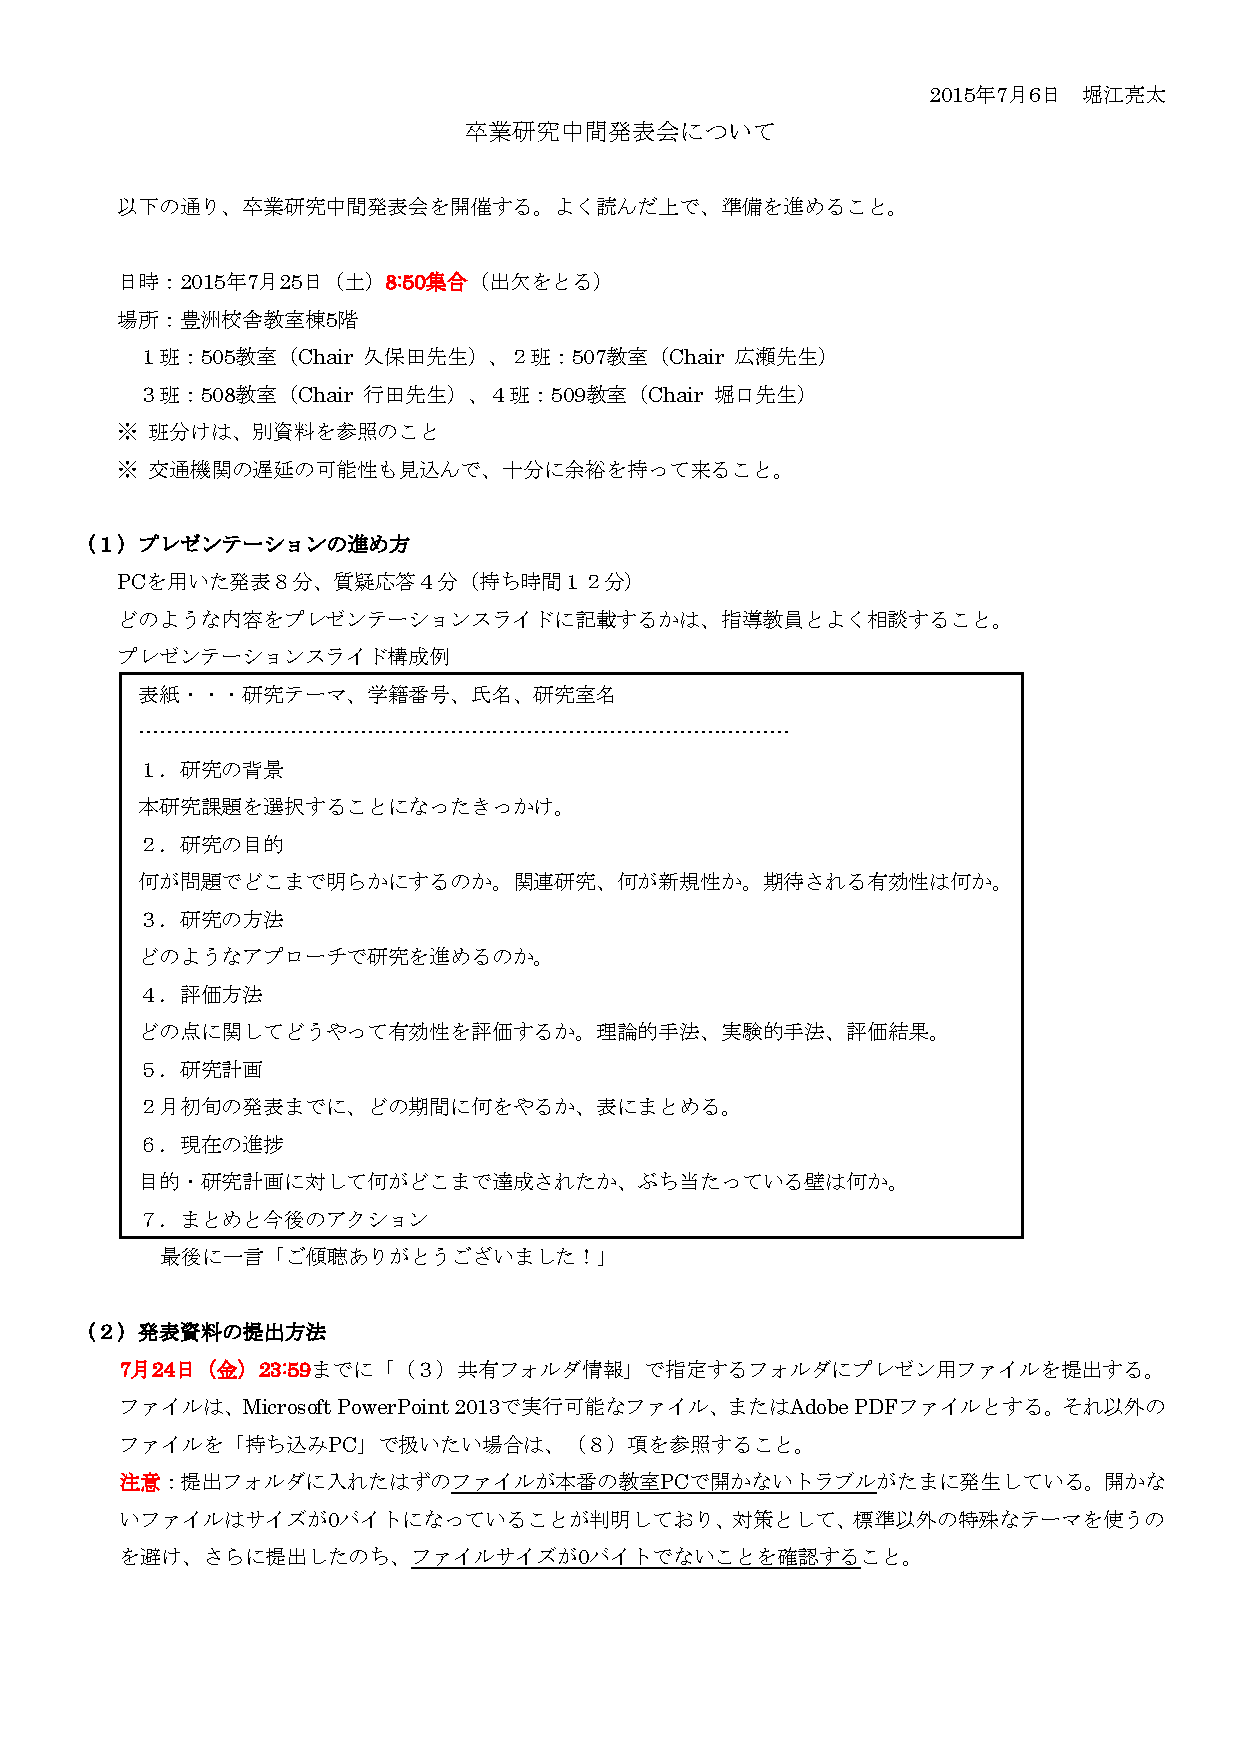
\includegraphics[width=0.65\linewidth]{chukanAnnounce.pdf}
\caption{2015年度卒業研究中間発表会案内文書}
\label{fig:chukanAnnounce}
\end{figure}
\begin{figure}[htbp]
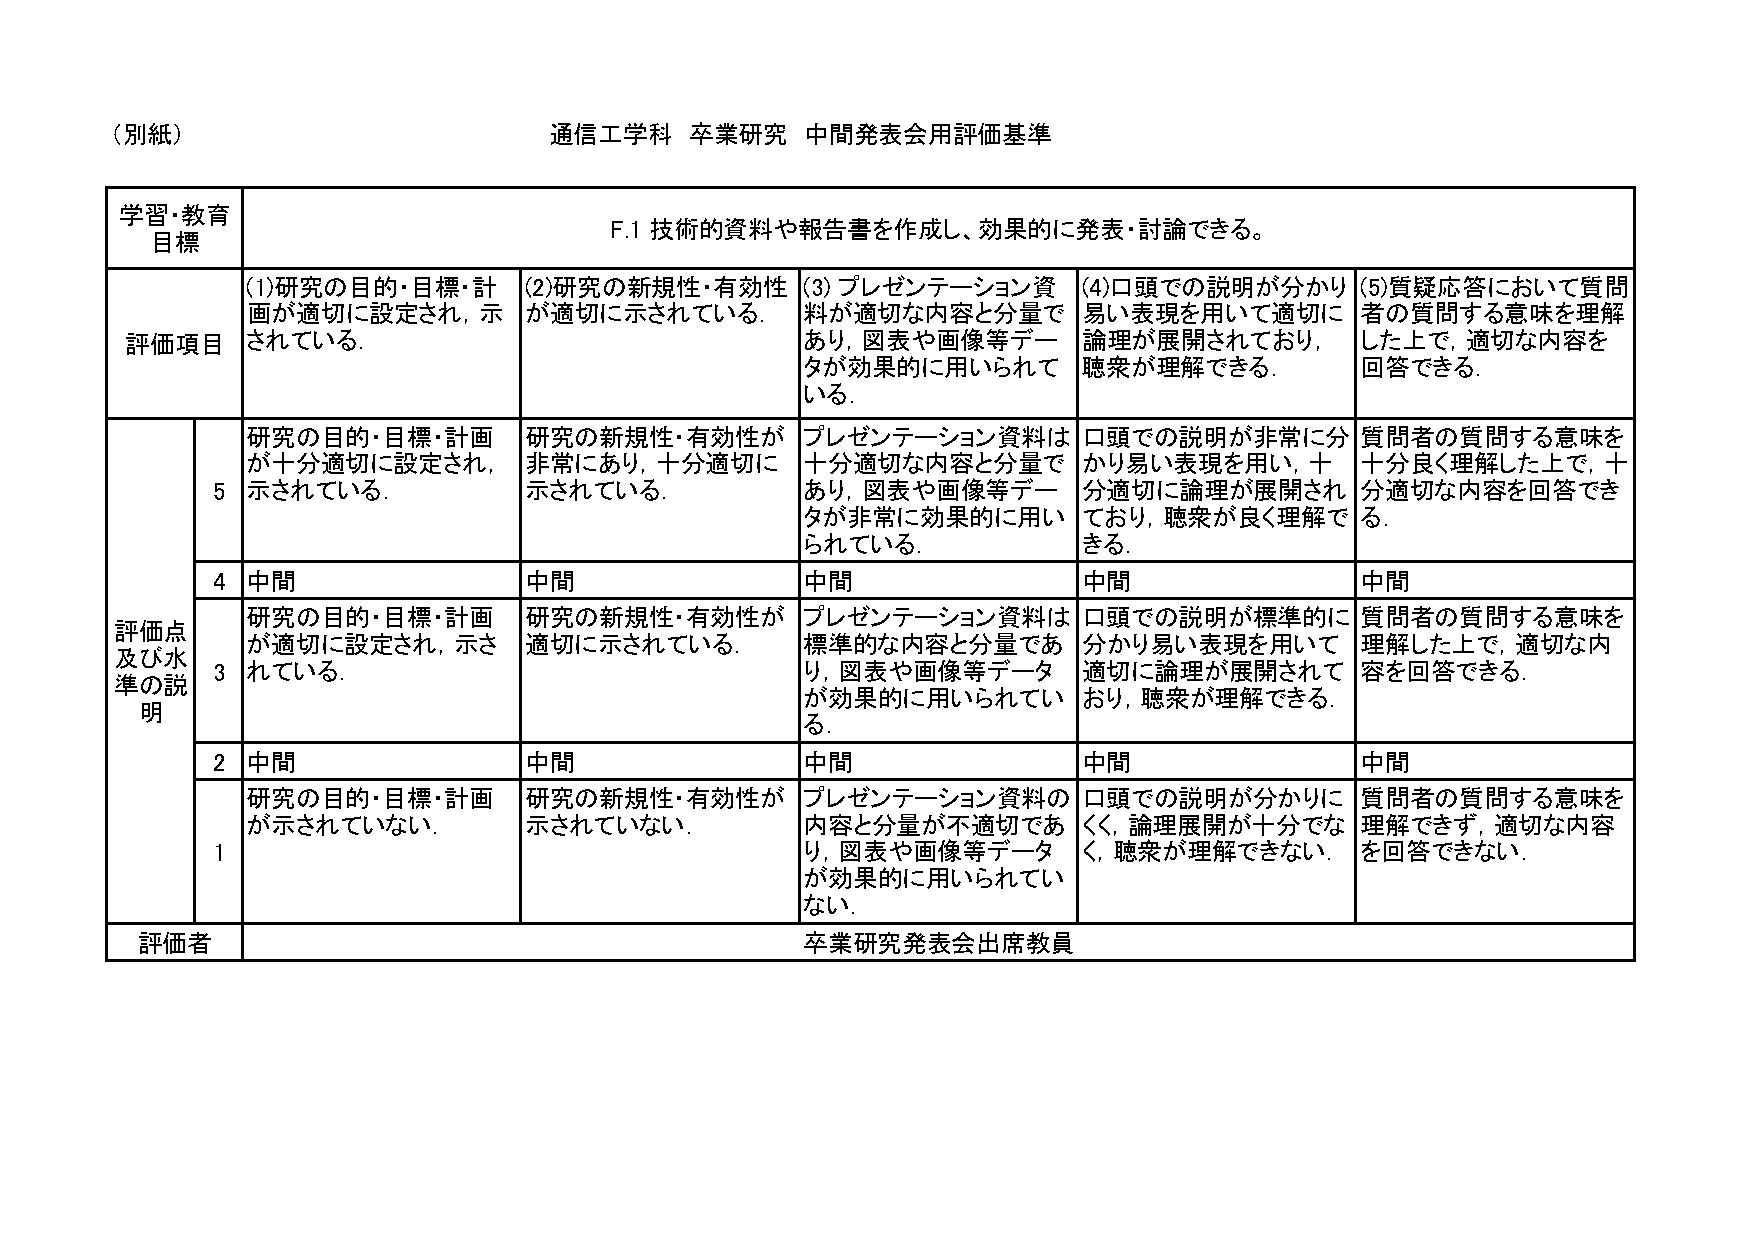
\includegraphics[width=\linewidth]{chukanLevel.pdf}
\caption{2015年度卒業研究中間発表会評価基準}
\label{fig:chukanLevel}
\end{figure}
%
%
%
\chapter{過去の卒業研究発表会関連配布資料}\label{chap:last}
%
%
%
\noindent
\begin{figure}[htbp]
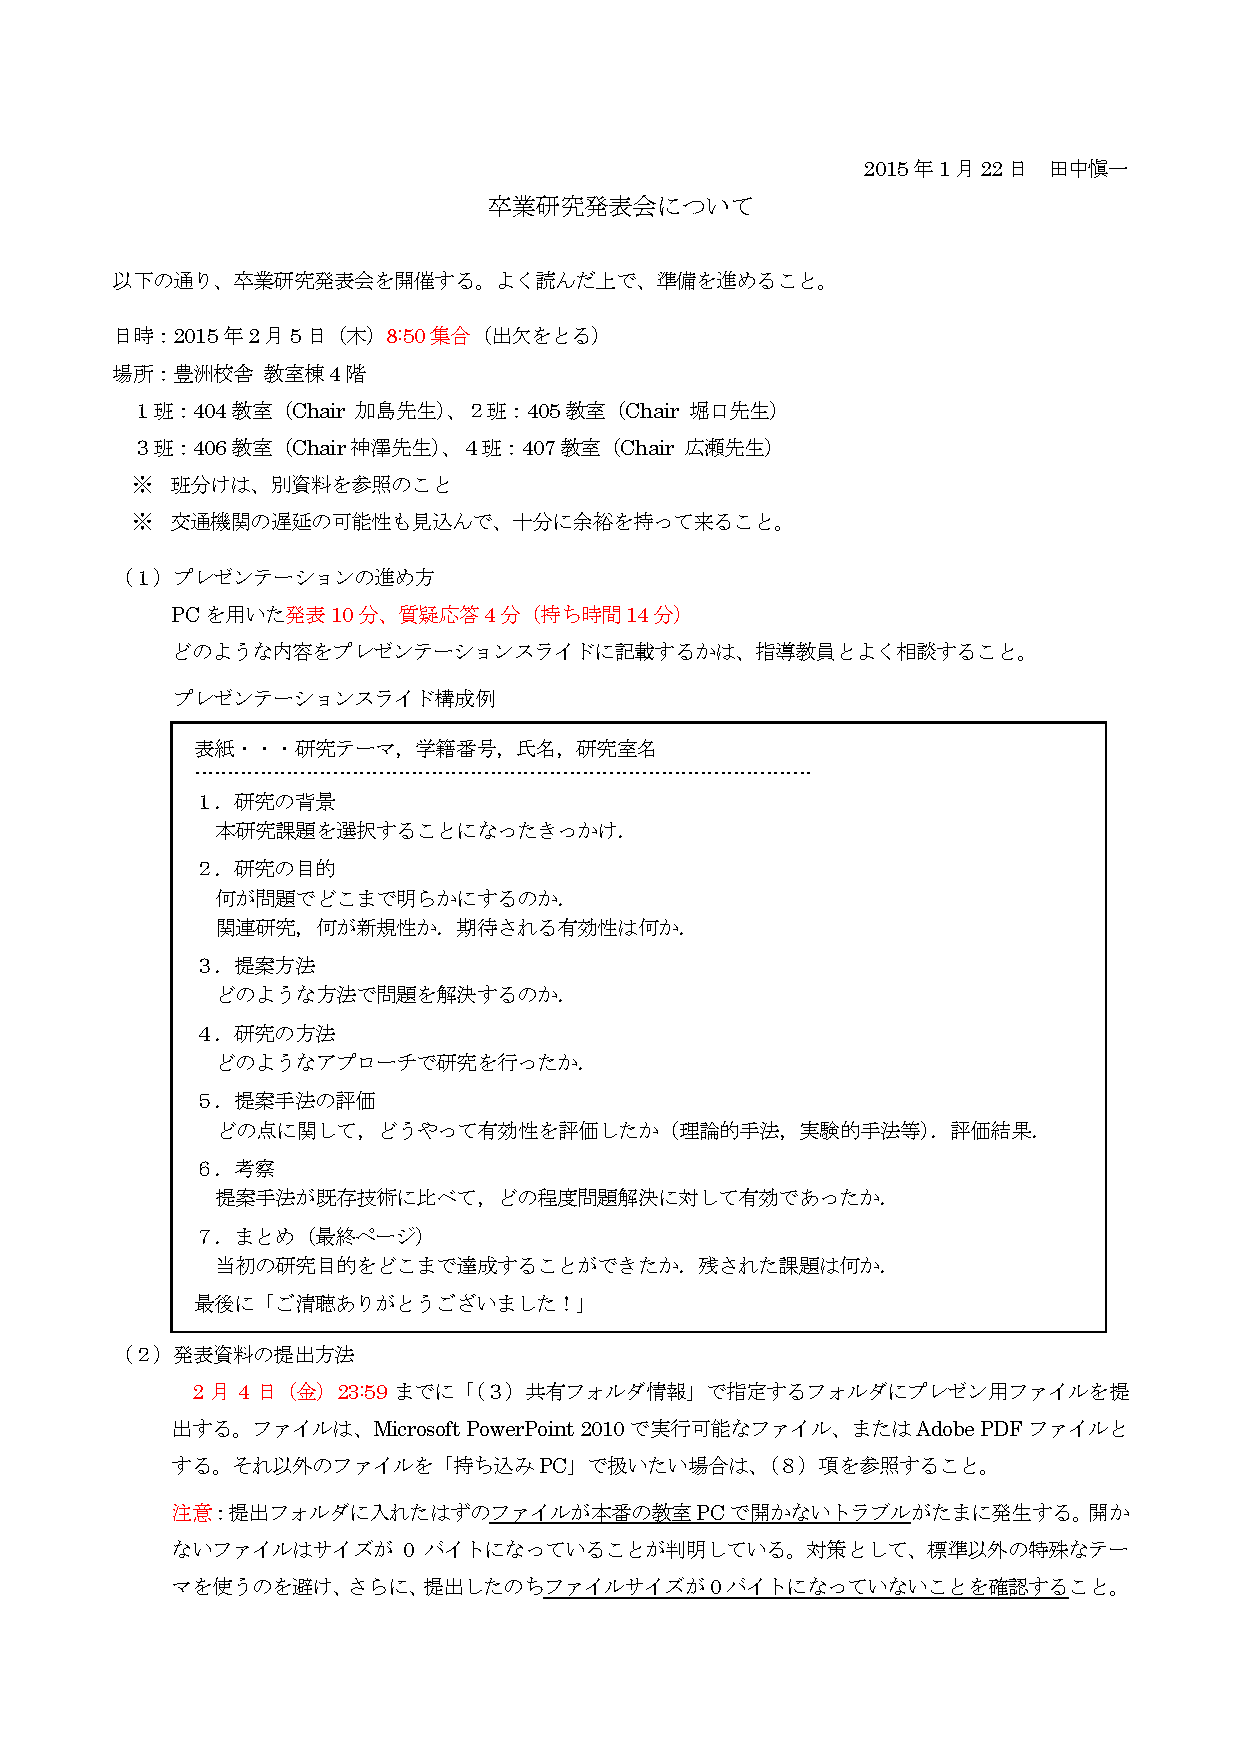
\includegraphics[width=0.65\linewidth]{presenAnnounce1.pdf}
\caption{2014年度卒業研究発表会案内文書}
\label{fig:presenAnnounce1}
\end{figure}
\begin{figure}[htbp]
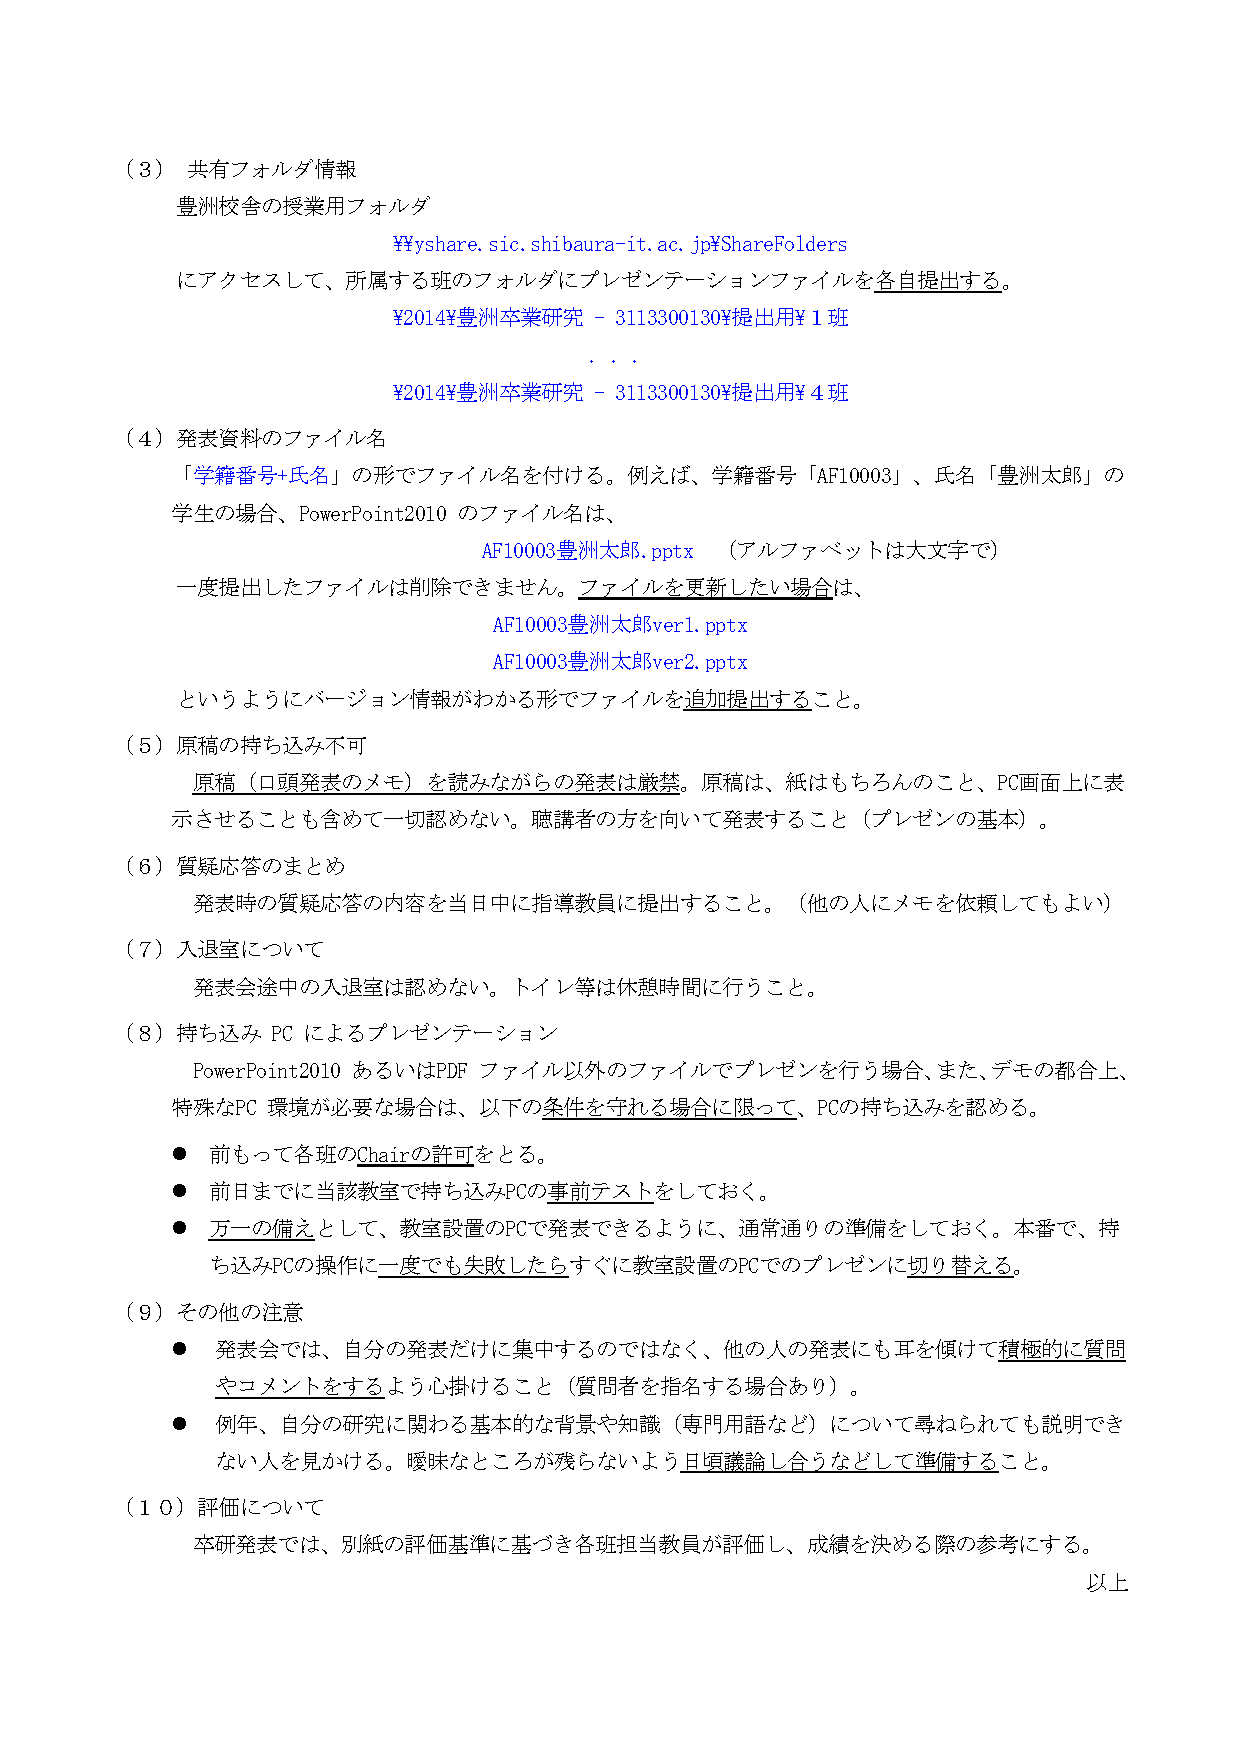
\includegraphics[width=0.8\linewidth]{presenAnnounce2.pdf}
\caption{2014年度卒業研究発表会案内文書の続き}
\label{fig:presenAnnounce2}
\end{figure}
\begin{figure}[htbp]
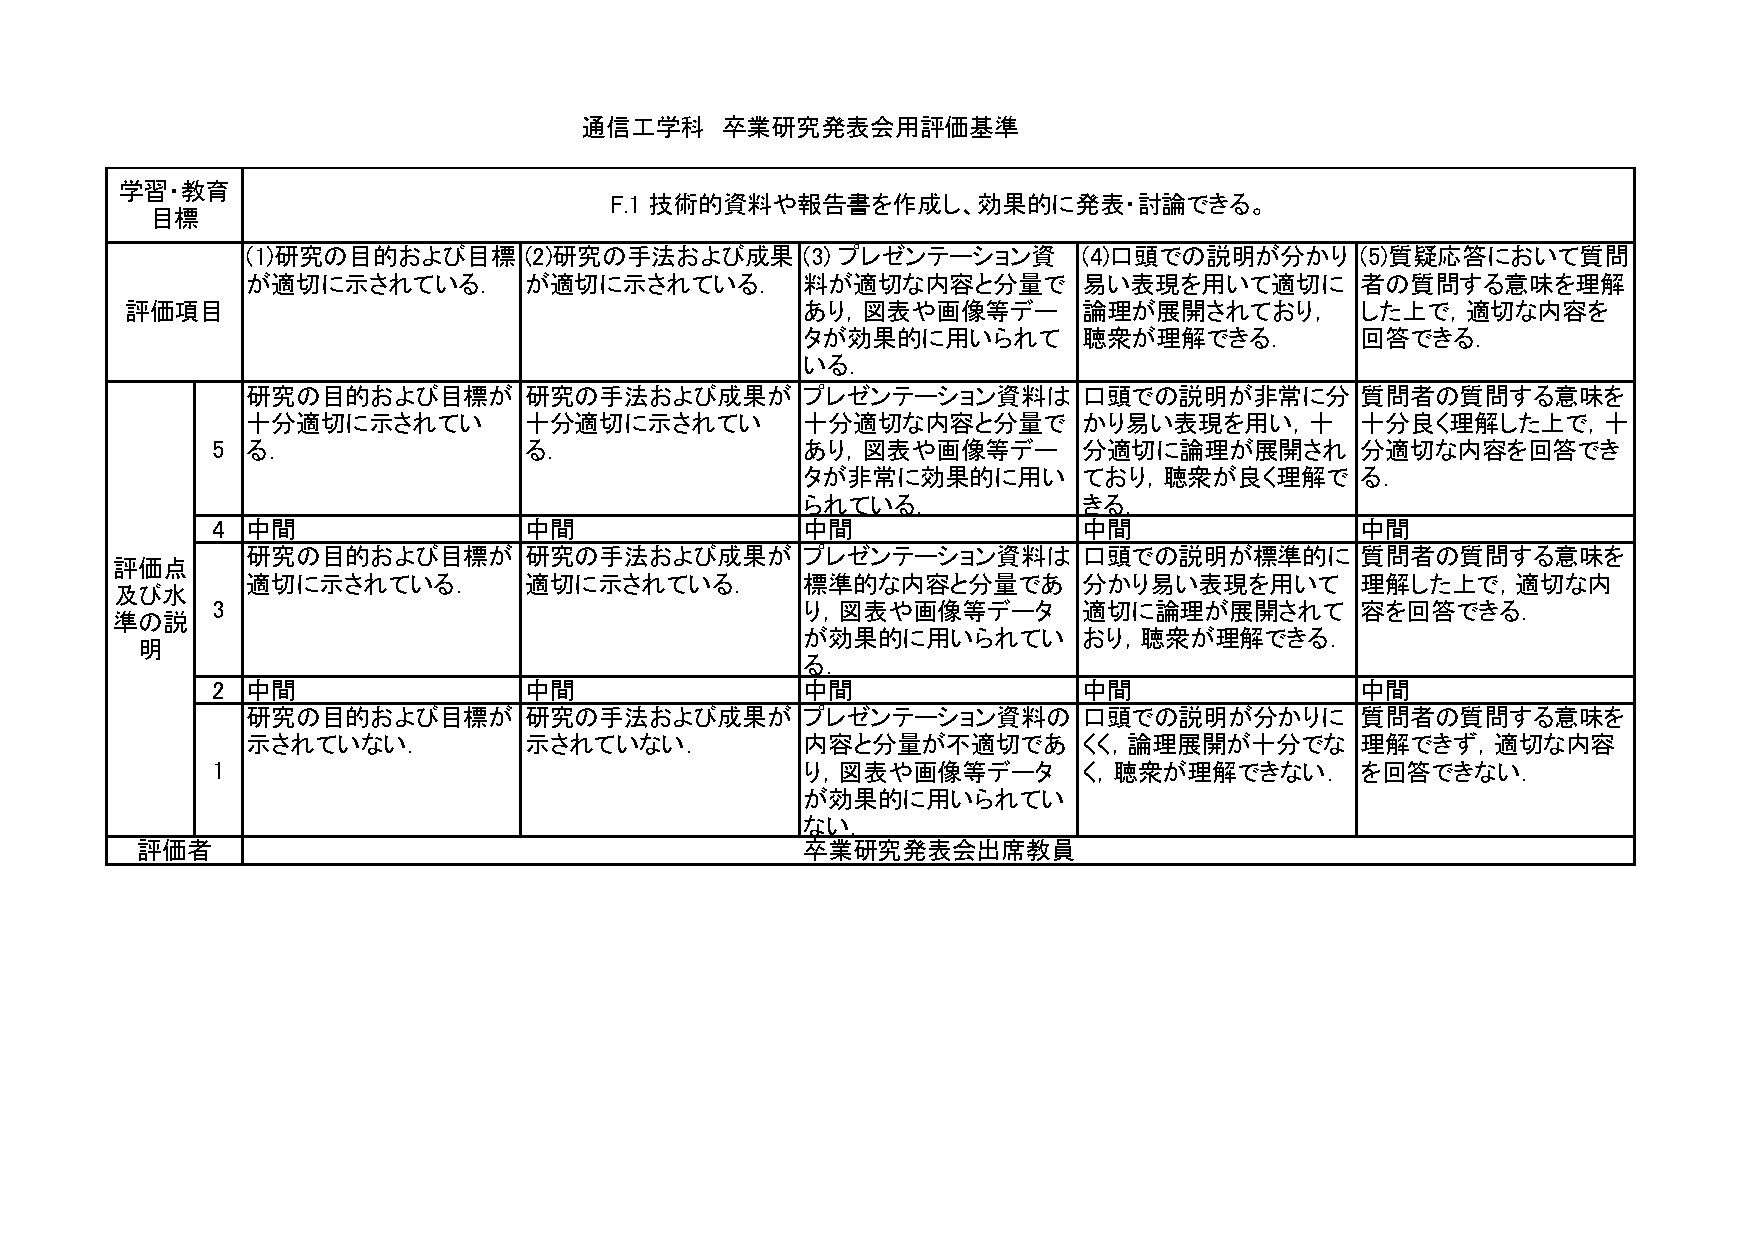
\includegraphics[width=\linewidth]{presenLevel.pdf}
\caption{2014年度卒業研究発表会評価基準}
\label{fig:presenLevel}
\end{figure}
\end{document}

